% Chapter Template

\chapter{Objetivos del sistema} % Main chapter title

\label{Chapter2} % Change X to a consecutive number; for referencing this chapter elsewhere, use \ref{ChapterX}

%----------------------------------------------------------------------------------------
%	SECTION 1
%----------------------------------------------------------------------------------------

\section{Objetivos}

Para la creación de contenido se permite el registro. Se contará con tanto con 3 perfiles de usuario: sin registro, con registro y administrador.
La aplicación cuenta a su vez con una version de Web y una version movil para Android con reproducción sincronizada entre ambos.
Los usuarios registrados tienen la posibilidad de administrar listas de reproducción públicas o privadas y a su vez el sistema genera listas de recomendaciones generales y para cada ususario.
A continuación se detalla el total de los requisitos.

\subsection{An\'alisis de requisitos preliminar}

\begin{itemize}
\item La aplicación permite reproducir canciones almacenadas en el repositorio.
\item La aplicación tendrá una versión para Android y otra para Web.
\item Existen 3 perfiles de usuario: registrados, no registrados y administrador.
\item Los usuarios registrados pueden generar y consumir contenido (canciones).
\item Los usuario no registrados solo pueden consumir contenido en la Web.
\item El sistema permite gestionar listas de reproducción públicas y privadas.
\item Se permite el login con la cuenta de usuario o con una cuenta Google mediante OAuth.
\item Verificación de cuenta. Esto supone un indicador gráfico en el perfil de usuario que anteriormente a verificado su identidad. La finalidad es garantizar la verdadera identidad del usuario.
\item En la versión movil, se permite almacenar la música en el dispositivo para poder acceder a esta sin conexión a internet.
\item La reproducción actual de un usuario se sincroniza en todos los dispositivos.
\item Integración con redes sociales, con la finalidad de compartir música, listas o perfiles en las RRSS.
\item Permite al usuario registrado generar sus propias listas de reproducción.

\item Un usuario registrado puede seleccionar 'Me gusta' en una canción.
\item Un usuario registrado puede suscribirse a otro usuario.
\item El sistema genera listas de reproducción segun las siguientes categorias: Género, Éxitos, Situación/Mood, País.
\item El sistema genera listas de reproduccion propias para cada usuario con recomendaciones según sus intereses.
\item El sistema genera listas de reproduccion con recomendaciones según geolocalización.
\item El sistema permite gestionar una lista privada de favoritos.
\item El sistema permite la búsqueda de canciones, albumes, listas y artistas.
\item El usuario administrador se utiliza para verificar, añadir o eliminar cuentas de usuarios.

\item Existe un servidor para el almacenamiento de canciones.
\item Los datos que se recogen en el formulario de registro son los siguientes: Nombre, Nick, Correo, Contraseña, Fecha de nacimiento, Biografía, Redes Sociales, Foto de perfil(opcional), País
\item Las canciones contienen los siguientes metadatos: Título, Idioma (opcional), número de reproducciones, número de 'Me gusta'.
\item La aplicación movil soportará Android 5.0
\item El sistema soporta los ficheros MP3, WAV, OGG.
\item La aplicación movil soporta la última versión de Firefox y Chrome.
\item El acceso al servidor se realiza a través de una API REST.
\end{itemize}

\subsection{Prototipo pantallas Android}
% ______________________
% Aqui comienza la tabla
\begin{tabular}{ p{6cm} p{6cm}}
\hline
\\
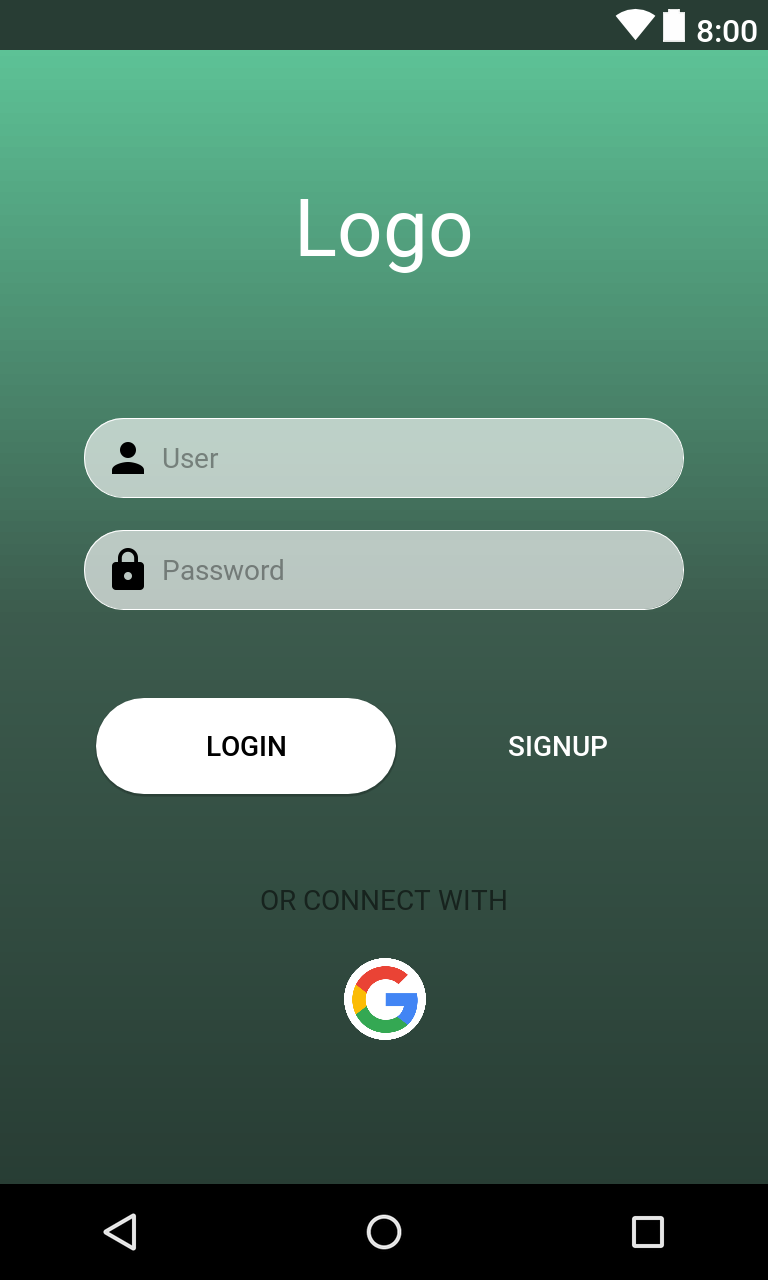
\includegraphics[width=6cm]{Figures/android/Login.png}
&
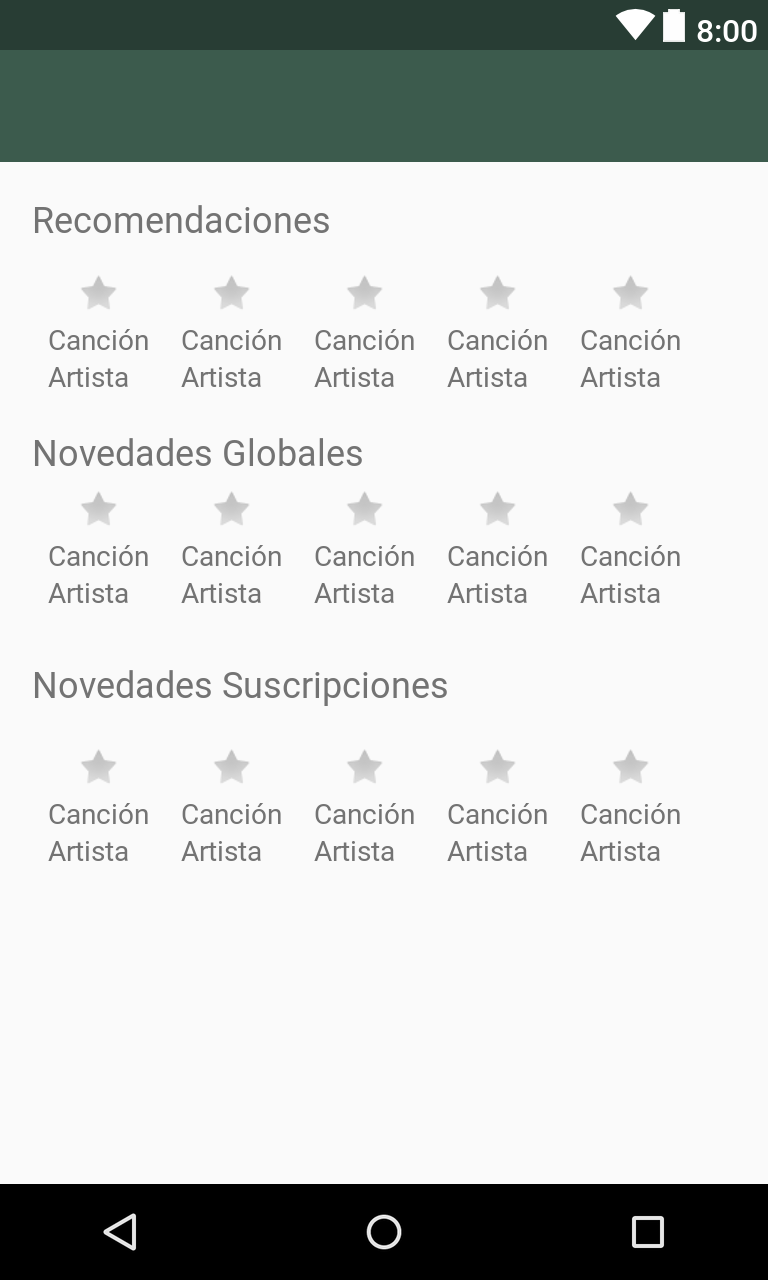
\includegraphics[width=6cm]{Figures/android/home.png} \\
\hline
\\
Pantalla de autentificación, en la que se permite tanto el acceso desde un usuario y contraseña de la aplicación así como desde una cuenta de Google. Esta es la primera pantalla que se abre en el caso de que el usuario no esté conectado
&
Pantalla principal de la aplicación en la cual se mostrarían diversos elementos de interés para el usuario, como pueden ser recomendaciones, novedades así como nuevas publicaciones que han producido artistas a los que se está suscrito.
Este esquema de pantalla también lo comparte una pantalla llamada explorar, la pantalla de novedades y la pantalla de recomendaciones.
En la pantalla explorar se mostrarían diversas listas de reproducción generadas por el sistema ( listas basadas en la ubicación del usuario, basadas en lo que escucha el usuario, basadas en lo que escucha el conjunto total de usuarios) así como los diferentes géneros musicales.  \\
\hline
\end{tabular}

\begin{tabular}{ p{6cm} p{6cm}}
\hline
\\
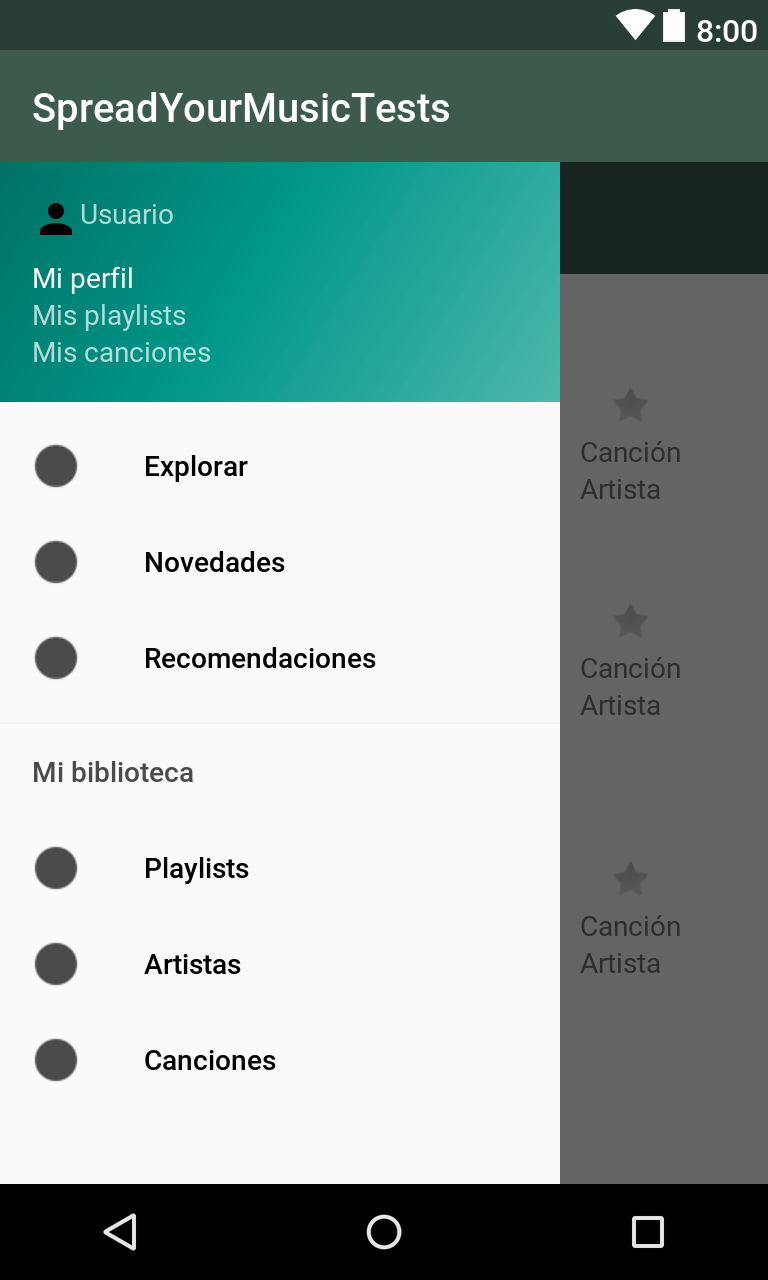
\includegraphics[width=6cm]{Figures/android/Home-NavigationDrawer.png}
&
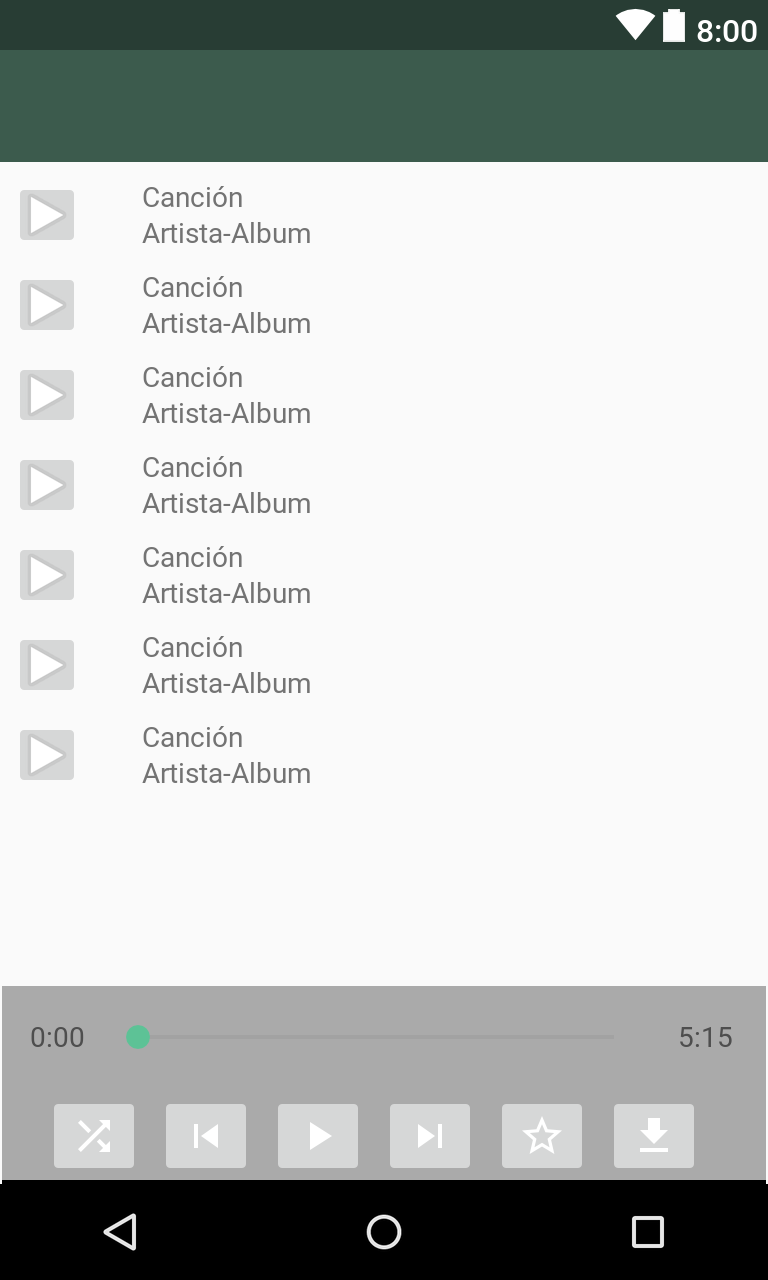
\includegraphics[width=6cm]{Figures/android/lista-reproductor.png} \\
\hline
\\
La forma de ir de una pantalla a otra en la aplicación sería mediante un panel lateral.
&
Desde cualquier pantalla se puede reproducir música, no es necesario que se esté en la pantalla del reproductor \\
\hline
\end{tabular}

\begin{tabular}{ p{6cm} p{6cm}}
\hline
\\
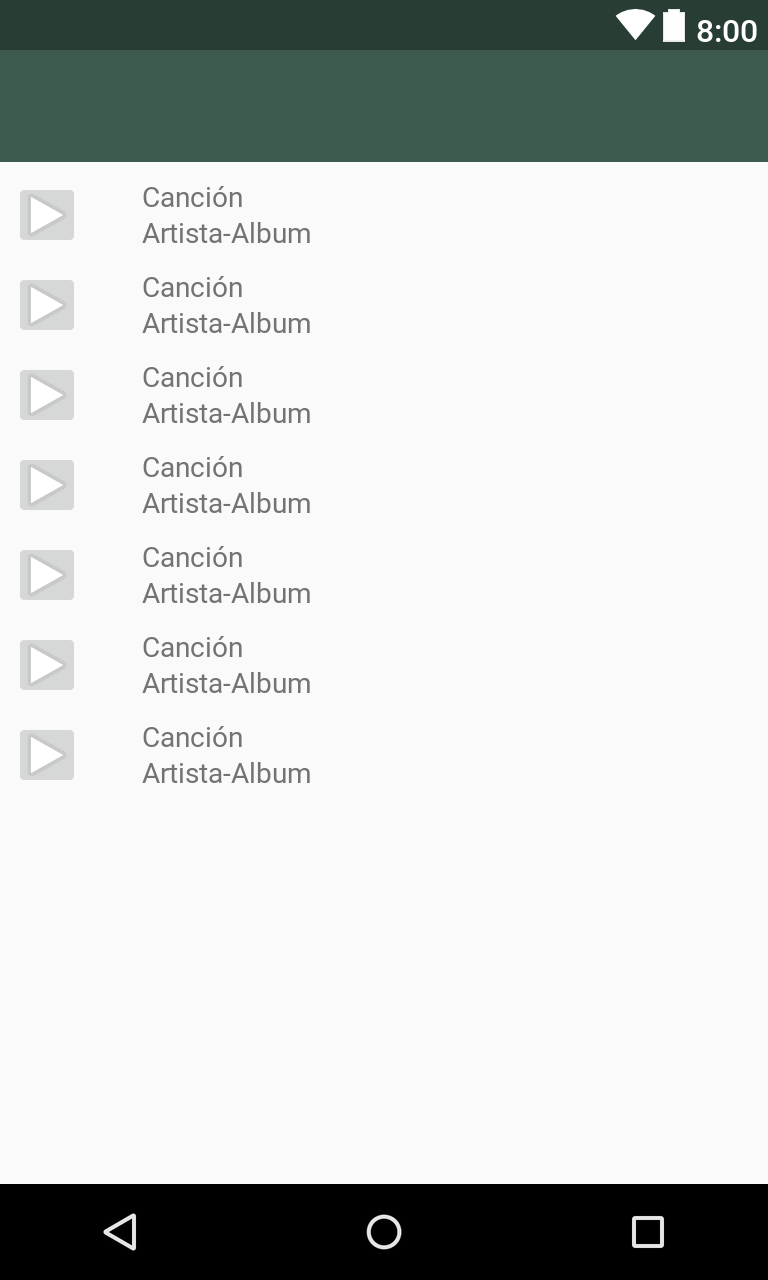
\includegraphics[width=6cm]{Figures/android/lista-no-personal.png}
&
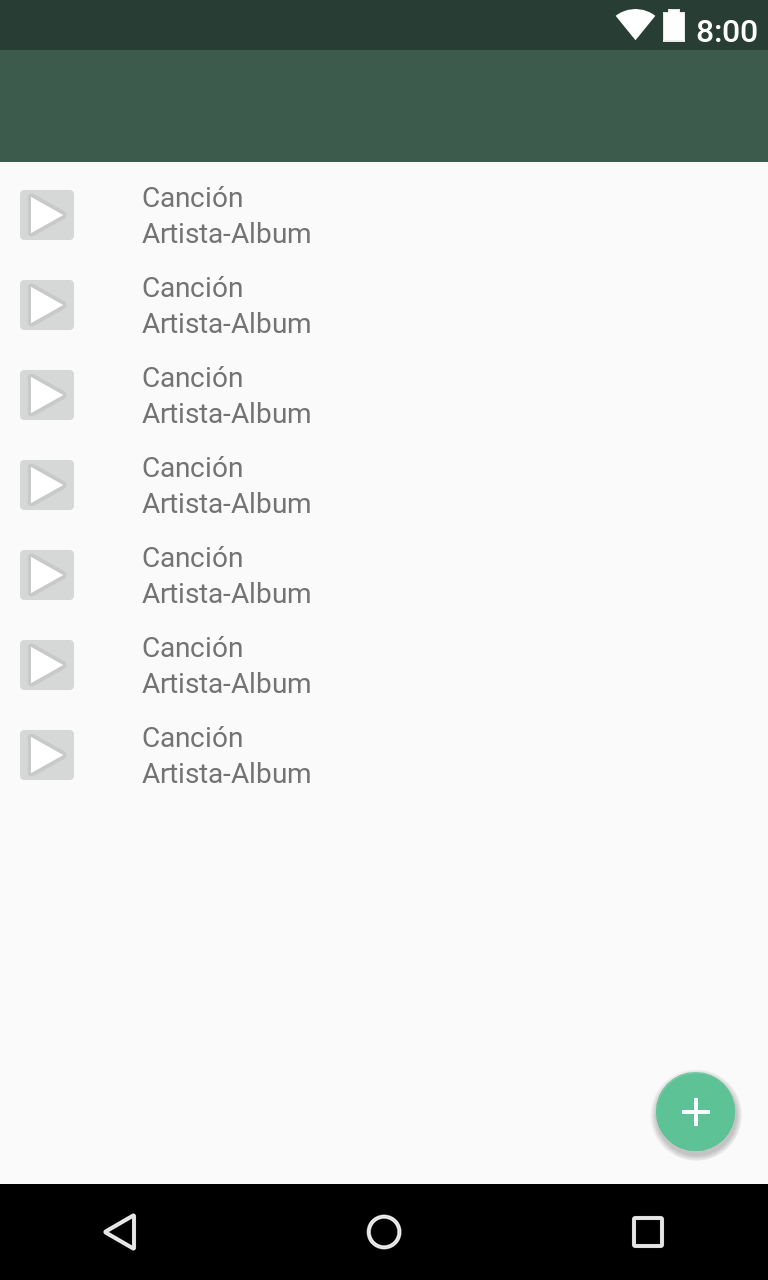
\includegraphics[width=6cm]{Figures/android/lista-personal.png} \\
\hline
\\
Lista de canciones, artistas o playlists. Este esquema de pantalla sería el que se produce al realizar una búsqueda o al acceder a las distintas categorías de mi biblioteca (playlist a las que sigues, canciones que te han gustado, artistas a los que sigues y canciones descargadas).
&
Este esquema de pantalla sería el que se produce al acceder a “Mis canciones” o “Mis playlists”.
Difiere del anterior en que permite añadir más elementos desde la pantalla. \\
\hline
\end{tabular}

\begin{tabular}{ p{6cm} p{6cm}}
\hline
\\
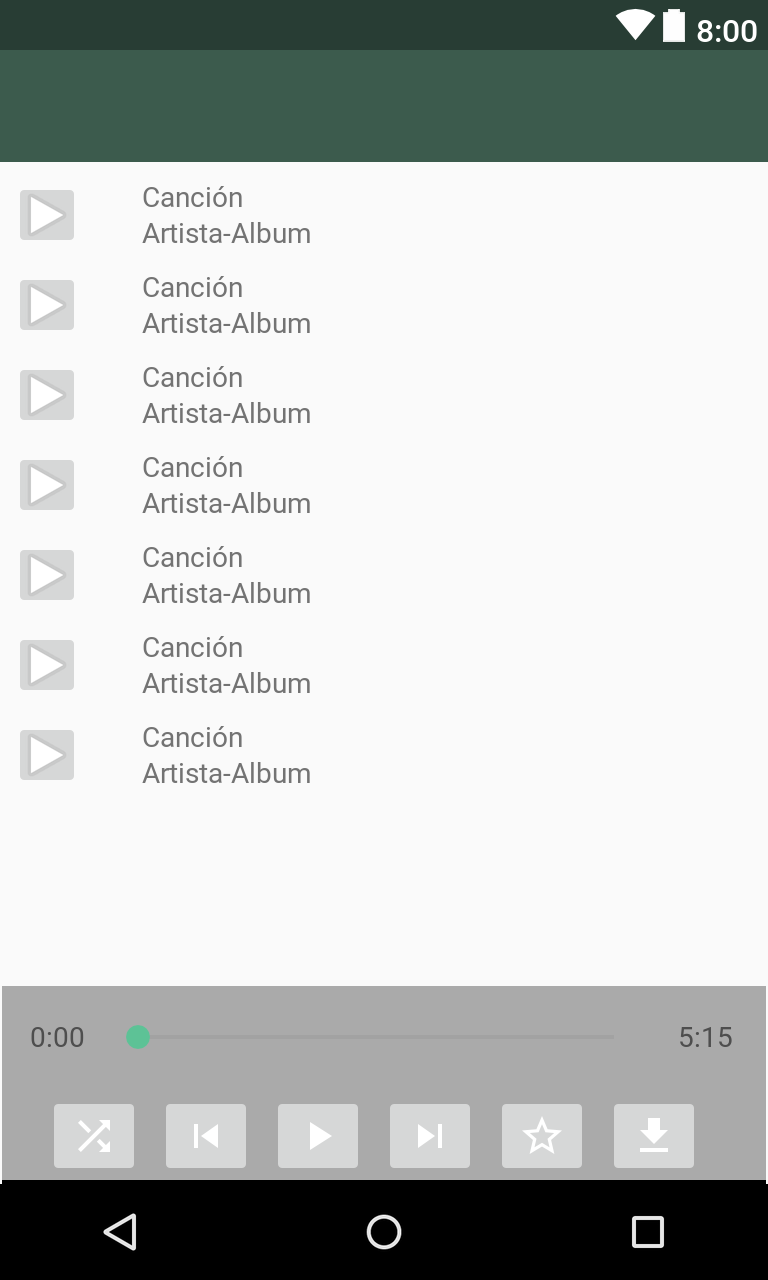
\includegraphics[width=6cm]{Figures/android/lista-reproductor.png}
&
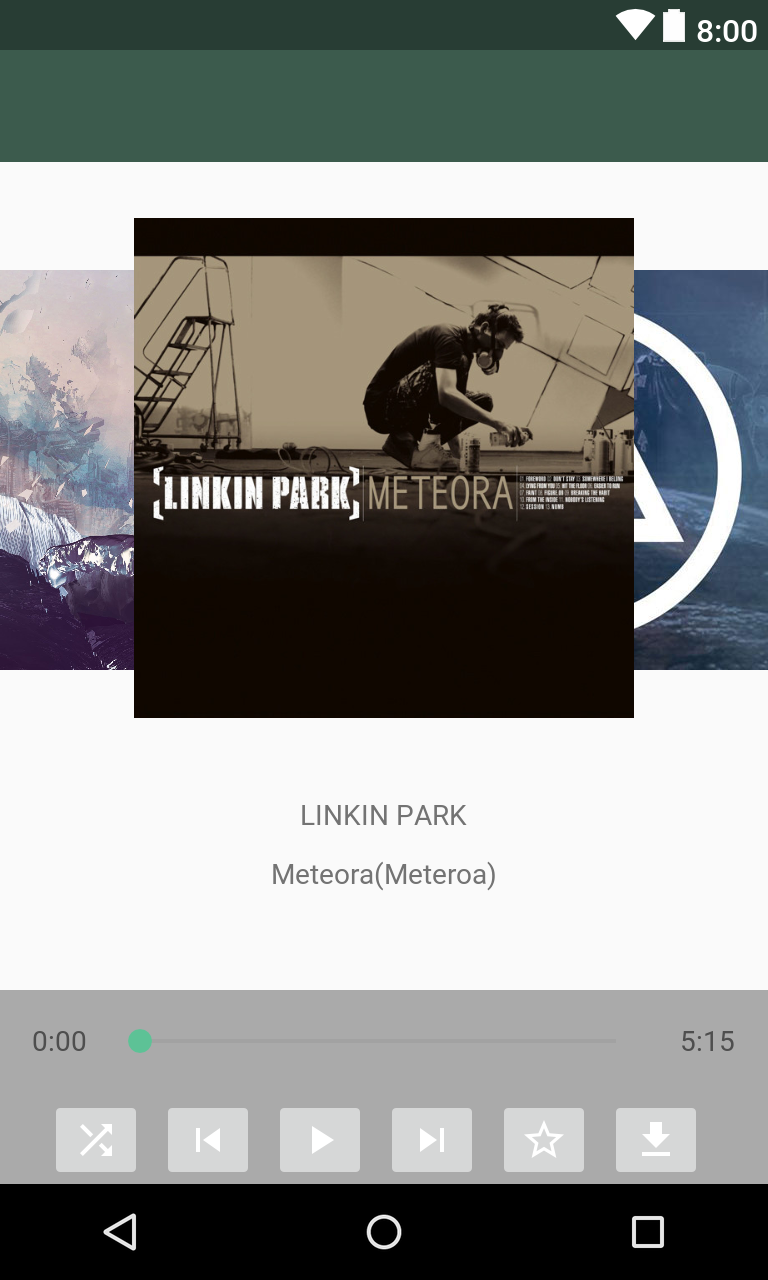
\includegraphics[width=6cm]{Figures/android/Reproductor.png} \\
\hline
\\
Desde cualquier pantalla se puede reproducir música, no es necesario que se esté en la pantalla del reproductor, en este caso se está reproduciendo desde una lista de canciones.
&
Pantalla del reproductor de música desde la que de puede descargar una canción, añadirla a favoritos ( opción de “me gusta”) . Desde esta pantalla también se podría compartirla en redes sociales. 
Esta pantalla se abre cuando se pulsa sobre una canción. \\
\hline
\end{tabular}

\begin{tabular}{ p{6cm} p{6cm}}
\hline
\\
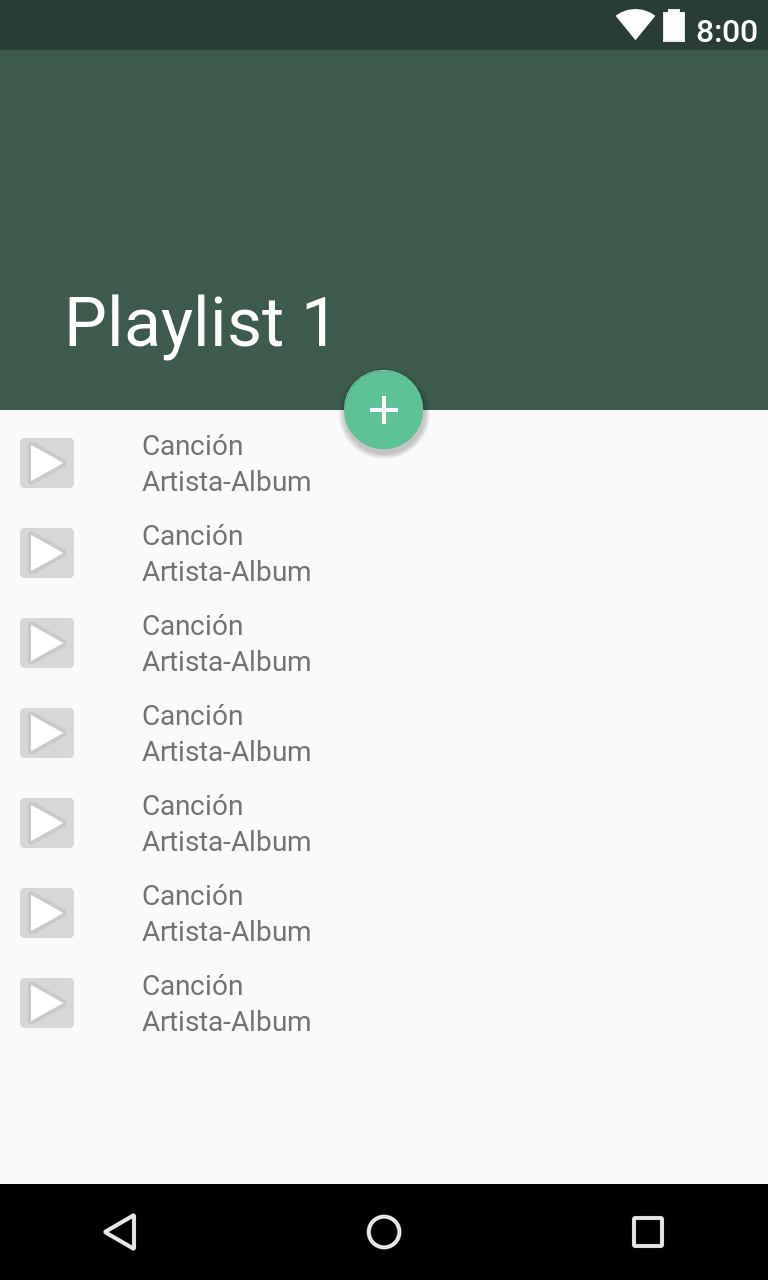
\includegraphics[width=6cm]{Figures/android/PlayList.png}
&
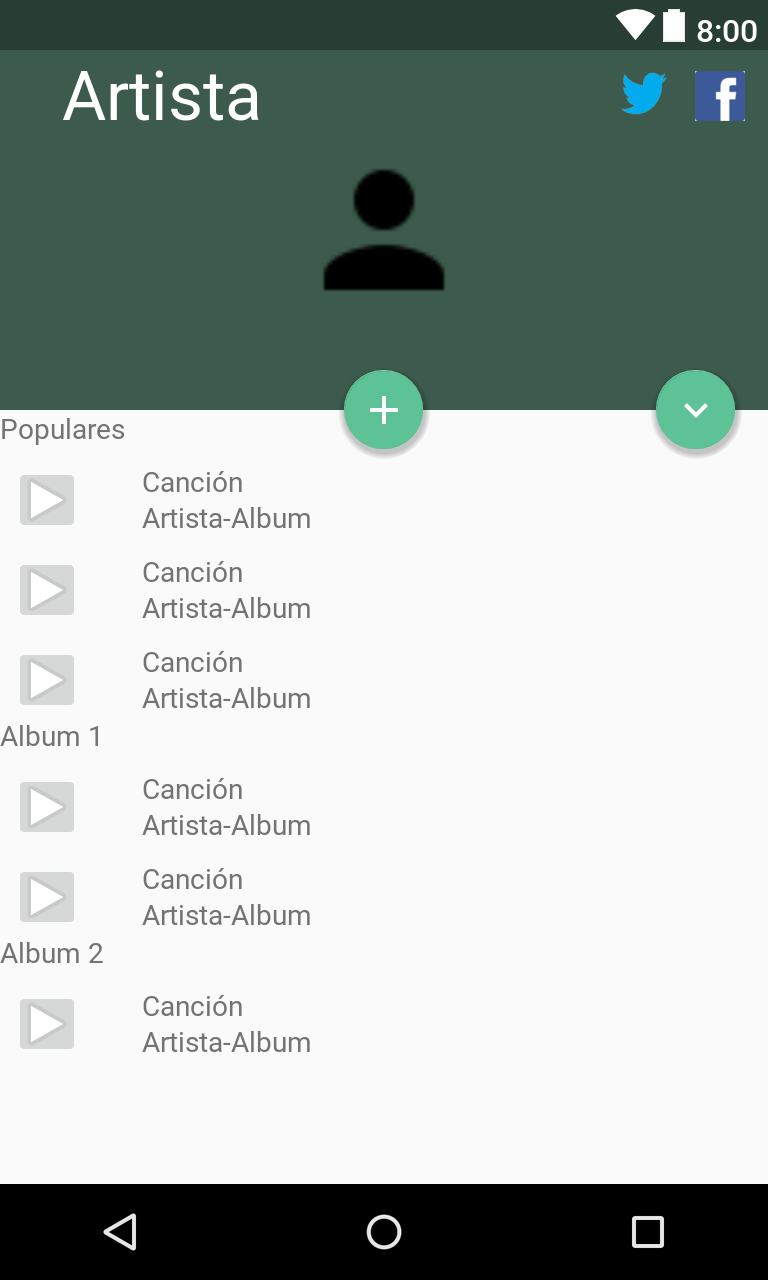
\includegraphics[width=6cm]{Figures/android/artista.png} \\
\hline
\\
Pantalla que aparece al pulsar sobre una playlist, desde la que se pueden ver las canciones que hay en dicha lista de reproducción, el creador de esta, así como suscribirse a ella.
&
Pantalla de perfil de usuario (perfil de artista), en la cual aparecen las canciones de un usuario clasificadas por álbumes, así como las listas de reproducción creadas por este usuario. También aparecen enlaces con redes sociales y la posibilidad de suscribirte a este usuario.
En esta pantalla también aparecerían estadísticas del usuario como pueden ser numero de seguidores o el número de visitas o “me gusta” que poseen sus canciones.  
\\
\hline
\end{tabular}
% ______________________
% Aqui termina la tabla

\vspace{1cm}
Las pantallas relacionadas con la subida de canciones y registro de usuario no se han incluido debido a que serían formularios.
La pantalla mi perfil no se ha incluido, aunque esta estaría compuesta por la información personal así como estadísticas de la cuenta (número de reproducciones totales recibidos, número de me gusta totales recibidos). También se daría la opción de editar la información personal.

\subsection{Prototipo pantallas Web}

\begin{tabular}{ p{6cm} p{6cm}}
	\hline
	\\
	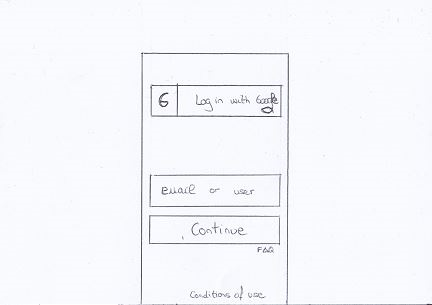
\includegraphics[width=6cm]{Figures/web/Login-web.png}
	&
	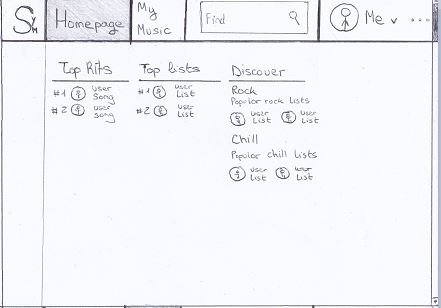
\includegraphics[width=6cm]{Figures/web/Lista-web.png} \\
	\hline
	\\
	Esta pantalla corresponde al inicio de sesión en la web y si es nuevo usuario, al registro del mismo.
	Se puede acceder mediante cuenta propia de la aplicación web (email o usuario) o mediante una cuenta de Google Plus.
	&
	Esta pantalla correspondería con la ventana principal en la aplicación, a traves de la cual se puede revisar la mejor música del momento recomendada para el usuario o acceder al resto de opciones (colección de álbunes, listas o pistas personales, búsquedas personalizadas o el propio perfil del usuario y su configuración).
	La aplicación permite al usuario reproducir la pista que desee haciendo click en sobre esta misma, procediendo así la aplicacíon a abrir en la parte inferior de la ventana la información de la pista y su estado actual (segundo de reproducción, si el usuario la ha marcado como favorita, etcétera).
	\\
	\hline
\end{tabular}

\begin{tabular}{ p{6cm} p{6cm}}
	\hline
	\\
	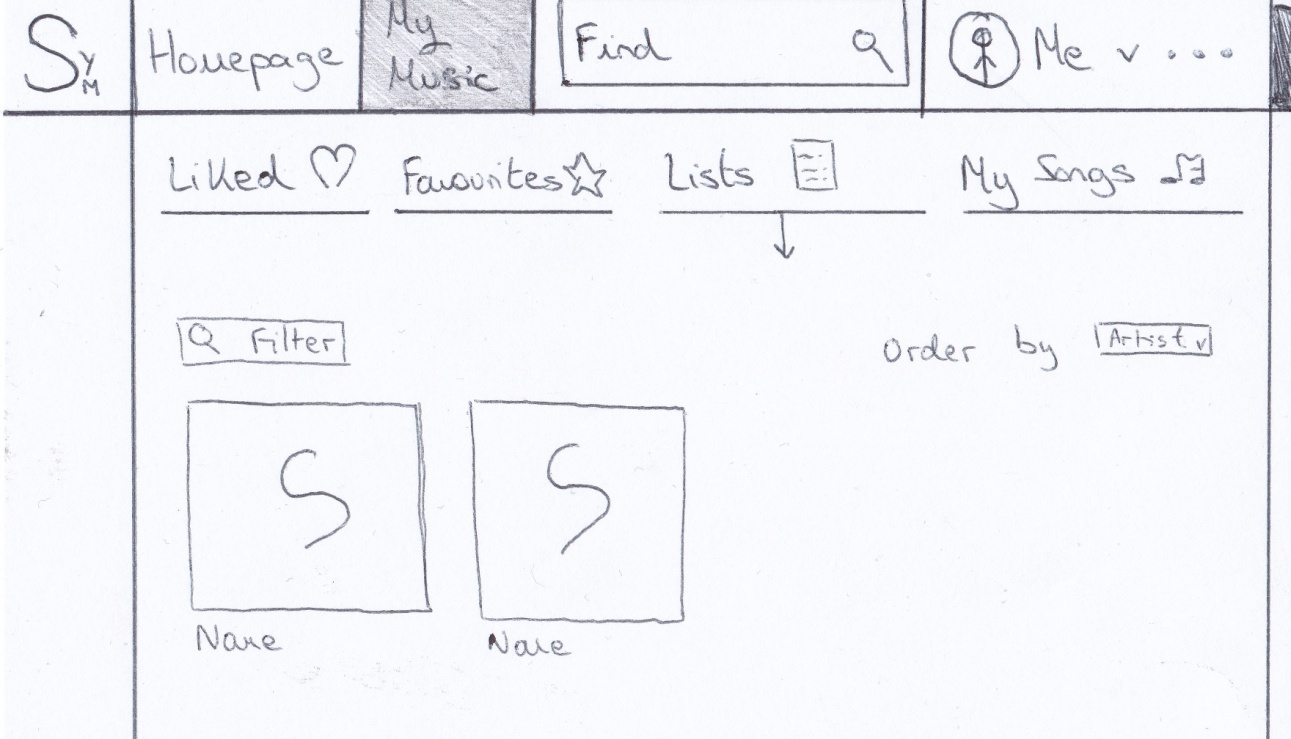
\includegraphics[width=6cm]{Figures/web/Main-web.png}
	&
	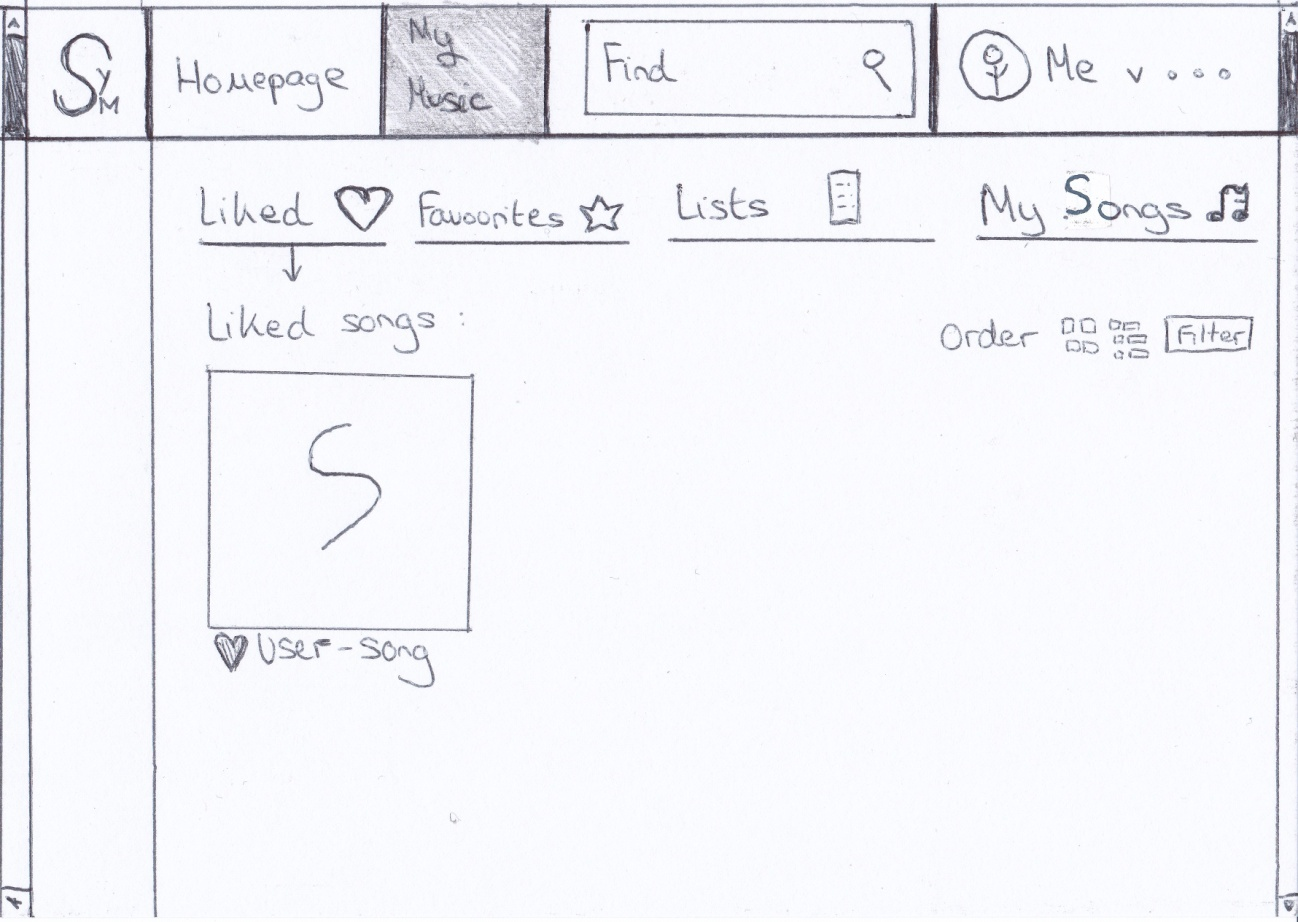
\includegraphics[width=6cm]{Figures/web/Reproduction-web.png} \\
	\hline
	\\
	Esta pantalla correspondería con tu colección de música en la aplicación, a traves de la cual se puede revisar la colección de álbunes, listas o pistas personales, así como las canciones que le gustan al usuario y sus canciones favoritas, ordenarlas o filtrarlas de manera personalizada.
	En este caso el usuario vería sus listas personales.
	La aplicación permite al usuario reproducir la pista que desee haciendo click en sobre esta misma, procediendo así la aplicacíon a abrir en la parte inferior de la ventana la información de la pista y su estado actual (segundo de reproducción, si el usuario la ha marcado como favorita, etcétera).
	&
	Esta pantalla correspondería con tu colección de música en la aplicación, donde a diferencia  de la anterior el usuario ha seleccionado visualizar las canciones que le gustan.
	La aplicación permite al usuario reproducir la pista que desee haciendo click en sobre esta misma, procediendo así la aplicacíon a abrir en la parte inferior de la ventana la información de la pista y su estado actual (segundo de reproducción, si el usuario la ha marcado como favorita, etcétera).
	\\
	\hline
\end{tabular}

\begin{tabular}{ p{6cm} p{6cm}}
	\hline
	\\
	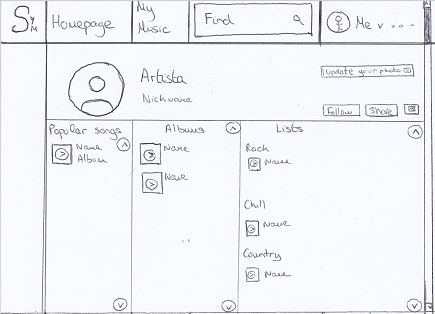
\includegraphics[width=6cm]{Figures/web/Artist-web.png}
	&
	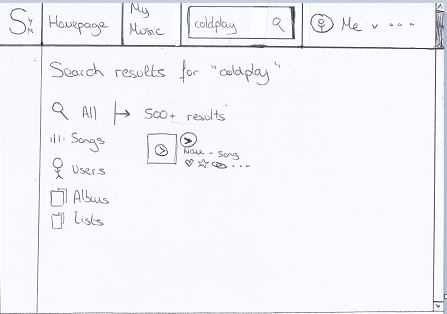
\includegraphics[width=6cm]{Figures/web/search-web.png} \\
	\hline
	\\
	Esta pantalla se correspondería con la vista general de un usuario donde este puede editar su foto de perfil si es el dueño de la cuenta o si es otro usuario suscribirse a las listas/pistas del usuario deseado.
	Se puede realizar scroll tanto en las canciones como listas o albunes del usuario.
	La aplicación permite al usuario reproducir la pista que desee haciendo click en sobre esta misma, procediendo así la aplicacíon a abrir en la parte inferior de la ventana la información de la pista y su estado actual (segundo de reproducción, si el usuario la ha marcado como favorita, etcétera).
	&
	Esta pantalla se correspondería con la obtención de resultados tras la búsqueda personalizada de un usuario que desea que le muestren toda la información disponible a cerca de las palabras clave seleccionadas, también se podría filtrar por pistas, listas, albunes o artistas disponibles.
	La aplicación permite al usuario reproducir la pista que desee haciendo click en sobre esta misma, procediendo así la aplicacíon a abrir en la parte inferior de la ventana la información de la pista y su estado actual (segundo de reproducción, si el usuario la ha marcado como favorita, etcétera).
	\\
	\hline
\end{tabular}